

\begin{frame}[fragile]
\frametitle{GPUs: Disillusion}
 \begin{block}{Computing Architecture Schematic}
  \begin{center}
   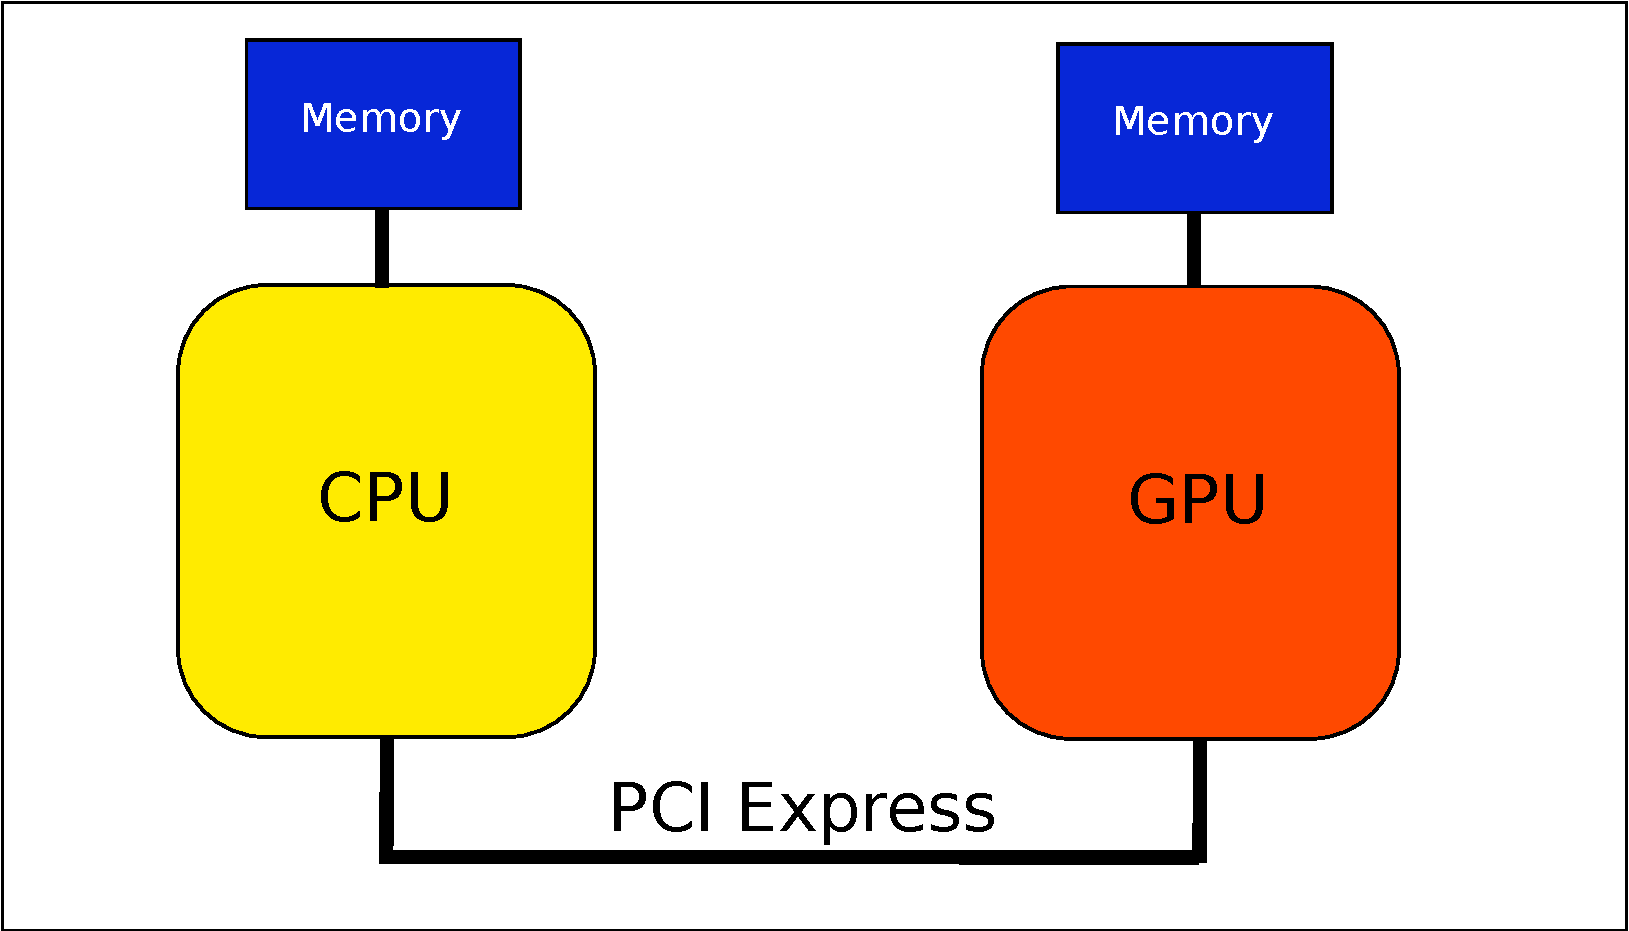
\includegraphics[width=0.8\textwidth]{figures/cpu-gpu-coarse.pdf}
  \end{center}

 
 \begin{itemize}
  \item \vspace*{1.03cm}
 \end{itemize}
 \end{block}

\end{frame}

\begin{frame}[fragile]
\frametitle{GPUs: Disillusion}
 \begin{block}{Computing Architecture Schematic}
  \begin{center}
   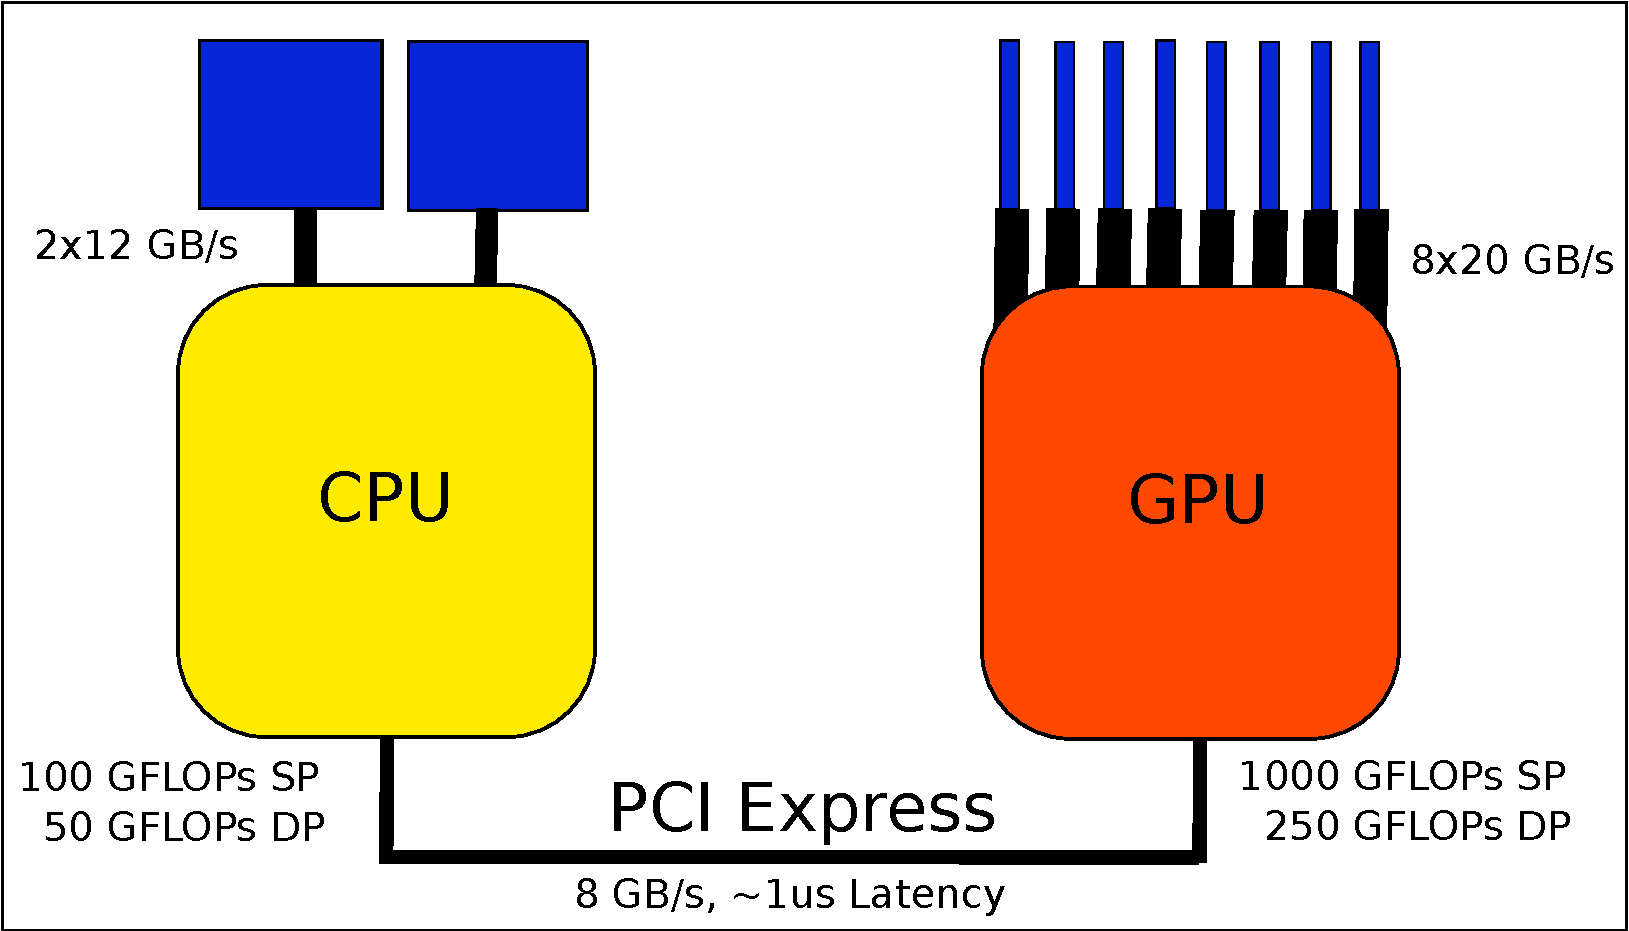
\includegraphics[width=0.8\textwidth]{figures/cpu-gpu-detail.pdf}
  \end{center}

 \begin{itemize}
  \item Good for large FLOP-intensive tasks, high memory bandwidth
  \item PCI-Express can be a bottleneck
  \item $\gg 10$-fold speedups (usually) not backed by hardware
 \end{itemize}
 \end{block}

\end{frame}


\begin{frame}{PETSc}
   \begin{center} (applet on architecture trends) \\[1em]
       {\footnotesize \url{http://www.eecs.berkeley.edu/~rcs/research/interactive\_latency.html}}
    \end{center}
\end{frame}





\begin{frame}{GPU Programming Approaches}
 
  \begin{block}{CUDA}
   \begin{itemize}
   \item Almost no additional code required
   \item Vendor-lock
   \item Relies on \lstinline|nvcc| being available
  \end{itemize}

  \end{block}

  \begin{block}{OpenCL}
  \begin{itemize}
   \item Additional boilerplate code required (low-level API)
   \item Broad hardware support (separate SDKs)
   \item No more development effort from NVIDIA
  \end{itemize}
  \end{block}

  \begin{block}{Directives}
   \begin{itemize}
    \item Annotate existing code with OpenMP-style Pragmas
    \item OpenACC and others
   \end{itemize}

  \end{block}

\end{frame}


\begin{frame}[fragile]{PETSc GPU Support}
 
  \begin{block}{NVIDIA Cusp/Thrust/CUSPARSE}
   \begin{itemize}
   \item Compile PETSc with CUDA support
   \item Use command line options to enable types, e.g.
    \begin{lstlisting}
 -vec_type cusp -mat_type aijcusp
    \end{lstlisting}
  \end{itemize}
  \end{block}

  \begin{block}{ViennaCL (OpenCL)}
  \begin{itemize}
   \item Compile PETSc with OpenCL support
   \item Use command line options to enable types, e.g.
    \begin{lstlisting}
 -vec_type viennacl -mat_type aijviennacl
    \end{lstlisting}
   \item Used for subsequent benchmarks
  \end{itemize}
  \end{block}

 \begin{center} No change in application code required! \end{center}
                                                        
\end{frame}


%%%% Which GPU is right for me?
\begin{frame}{Which Accelerator is Right for Me?}
 
  \begin{block}{Available Accelerators (Rough Sketch)}

   \begin{center}
    \begin{tabular}{|l|c|c|c|c|c|}
     \hline
      Name             & TFLOP/s & RAM (GB) & GB/s & TDP & Price \\
     \hline
     NVIDIA GTX 580    & 1.5/$\sim$0.2 & 1.5-3.0 & 192 & 244 & \$500   \\
     NVIDIA GTX Titan  & 4.5/1.3  & 6.0     & 288 & 250 & \$$\sim$1k \\
     NVIDIA Tesla 2050 & 1.3/0.5  & 3.0-6.0 & 150 & 225 & \$$\sim$2k \\
     NVIDIA K20        & 3.5/1.2  & 5.0     & 200 & 220 & \$$\sim$3k \\
     \hline
     AMD HD 7970       & 3.5/$\sim$0.9 & 3.0-6.0 & 264 & 250 & \$550 \\
     AMD FirePro W9k   & 4.0/1.0  & 6.0     & 264 & 274 & \$$\sim$3k \\
     \hline
     Intel Xeon Phi    & $\sim$2.0/$\sim$1.0 & 8 & 320 & 225 & \$$\sim$3k \\
     \hline
     \hline
     Intel Xeon E5-264x  & 0.2/0.1  & $\sim$64 & $\sim$48 & 100 & \$$\sim$1k \\
     \hline
   \end{tabular}
   \end{center}
  \end{block}

  %\visible<2>{
  \begin{block}{PETSc Considerations}
   \begin{itemize}
    \item Single precision performance doesn't matter
    \item Essentially all kernels memory bandwidth limited
    \item Memory access patterns rather irregular
   \end{itemize}
  \end{block}
  %}

\end{frame}


